\section{Alcance}

Definir con precisión el alcance es fundamental para asegurar que el desarrollo se ajuste a los objetivos propuestos y se realice dentro de los recursos y tiempos establecidos. Para ello, en esta sección se delimitarán las funcionalidades, exclusiones y limitaciones que se esperan en este proyecto.

\subsection{Funcionalidades Incluidas}

En la plataforma web se ofrecen las siguientes funcionalidades principales:

\begin{itemize}
    \item \underline{Autenticación segura} mediante las credenciales de \textit{Spotify}.
    \item \underline{\textit{Home} o Panel Inicial} donde se muestran la información básica de la cuenta.
    \item Análisis detallado y visualizaciones \underline{gráficas avanzadas, interactivas y actualizadas} de sus datos musicales.
    \item Interfaz \underline{adaptativa, intuitiva y responsiva}.
    \item \underline{Cierre de sesión seguro}.
\end{itemize}

\subsection{Exclusiones}

Para establecer expectativas claras sobre el alcance del proyecto, se detallan a continuación las funcionalidades que \textbf{no} serán incluidas en la plataforma web:

\begin{itemize}
    \item No se desarrollarán \underline{aplicaciones nativas de otras plataformas} como móvil, PC, Mac o Linux; el acceso será exclusivamente a través de la web.

    \item Aunque se seguirá un diseño intuitivo, no se implementarán funcionalidades específicas de \underline{accesibilidad avanzadas} como compatibilidad con lectores de pantalla o navegación por teclado.

    \item La plataforma se enfoca exclusivamente en la integración con \textit{Spotify}; se excluyen todos los \underline{otros servicios de streaming} como \textit{Apple Music}, \textit{Deezer}, etc.

    \item No se \underline{almacenarán de forma persistente datos personales} del usuario en servidores propios más allá de lo necesario para la sesión actual; todos los datos se obtendrán directamente de la API de \textit{Spotify} y se manejarán en tiempo real.

    \item Se excluye el desarrollo de funcionalidades relacionadas con la \underline{interacción social} (envío de mensajes, compartir estadísticas, rankings entre usuarios, etc.) dentro o a través de la plataforma, ya que superarían el alcance recogido dentro de un TFG.

          % * COMPROBAR SI SE HAN IMPLEMENTADO O NO ESTAS FUNCIONALIDADES * %

          % * \item \textbf{Integración con Redes Sociales}: No se implementarán opciones para compartir estadísticas o visualizaciones directamente en redes sociales como Facebook, Twitter o Instagram.

          % * \item \textbf{Exportación de Datos o Estadísticas}: No se incluirá la opción de exportar los datos o estadísticas a formatos externos como PDF, CSV o imágenes descargables.

          % * \item \textbf{Soporte Multilenguaje}: La interfaz de usuario estará disponible únicamente en español y no se ofrecerá soporte para otros idiomas.

\end{itemize}

\subsection{Limitaciones}

Durante el desarrollo del proyecto, se han identificado las siguientes limitaciones que han afectado al alcance y a las funcionalidades de la web:

\begin{itemize}
    \item Las políticas de seguridad de \textit{Spotify} impiden el \underline{almacenamiento persistente de datos} personales, limitando funcionalidades que requieran conservar información del usuario entre sesiones.

    \item El procesamiento de los datos se ve limitado por los \underline{recursos computacionales} que la nube de \textit{Vercel} ofrece, descartando técnicas avanzadas como el aprendizaje automático.

    \item El \underline{tiempo y los recursos disponibles} para el desarrollo del proyecto son finitos, lo que ha obligado a priorizar funcionalidades esenciales y descartar características adicionales.

    \item Al hacer uso de una API de terceros, todas las funcionalidades necesitan una \underline{conexión} \underline{activa a Internet} para poder funcionar de manera correcta.
\end{itemize}

\section{Gestión de Tareas}

Una vez definido el alcance, es necesario detallar las tareas requeridas para el desarrollo del proyecto. En esta sección se caracterizará todo lo necesario en relación a las tareas, incluyendo su definición, relaciones y tiempos asignados, para asegurar una gestión estructurada y alineada con los objetivos del proyecto.

\subsection{Descripción de Tareas}

Para gestionar de manera efectiva el conjunto de actividades, se ha elaborado una Estructura de Desglose de Trabajo (EDT). Esta EDT (figura \ref{fig:edt}) proporciona una visión general de las principales áreas de trabajo, desglosando el proyecto en paquetes específicos que abarcan cada tarea esencial, facilitando así la gestión.

En este caso, el proyecto se organiza en cinco áreas principales, que abarcan todas las fases del desarrollo de la aplicación; abordando tanto las tareas relacionadas con la creación de la aplicación en sí misma (el producto final) como aquellas enfocadas en la gestión y redacción del proyecto para su documentación. Esta estructura garantiza una distribución clara de las tareas, cubriendo tanto los aspectos técnicos como los organizativos.

\begin{figure}[H]
    \centering
    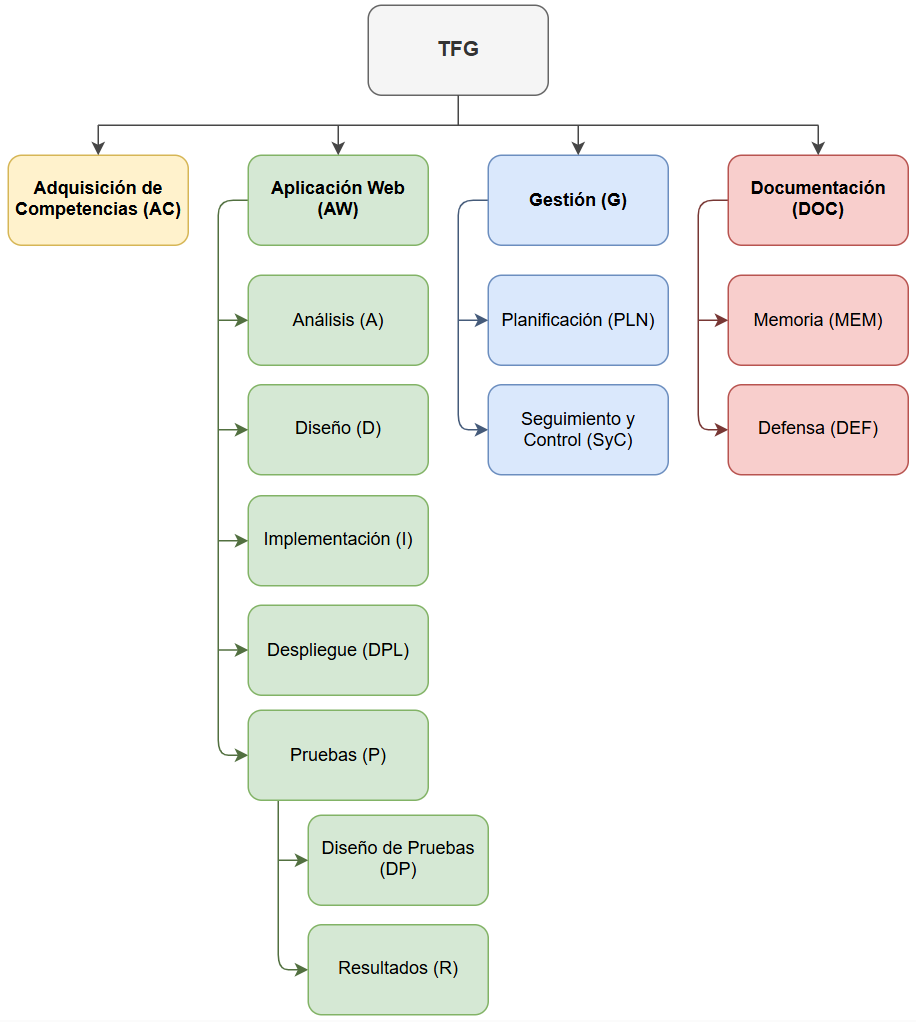
\includegraphics[width=\textwidth]{figures/edt.png}
    \caption{Diagrama EDT con los paquetes de trabajo del proyecto.}
    \label{fig:edt}
\end{figure}

A continuación se detalla cada paquete de trabajo y las tareas correspondientes contenidas en cada una:

\subsubsection{Adquisición de Competencias (AC):}

Este paquete de trabajo incluye todas las tareas necesarias para adquirir el conocimiento sobre las tecnologías y herramientas clave para el desarrollo del proyecto.

\begin{itemize}
    \item \textbf{AC.1:} Aprender \textit{TypeScript}, \textit{React.js} y \textit{Next.js} para el desarrollo de la aplicación web.
    \item \textbf{AC.2:} Estudiar el uso de \textit{Vercel} para el hosting y despliegue de la aplicación.
    \item \textbf{AC.3:} Hacer un reconocimiento inicial de la \textit{Web API} de \textit{Spotify}.
\end{itemize}

\subsubsection{Aplicación Web (AW):}

En este paquete se engloban todas las fases de desarrollo de la aplicación web, desde la planificación inicial hasta el despliegue final.

\begin{itemize}
    \item \textbf{Análisis (A):}
          \begin{itemize}
              \item \textbf{AW.A.1:} Estudiar y analizar en profundidad la \textit{Web API} de \textit{Spotify} para determinar el alcance y sus limitaciones.
              \item \textbf{AW.A.2:} Definir los requisitos funcionales y no funcionales del sistema.
              \item \textbf{AW.A.3:} Desarrollar los principales casos de uso del sistema.
          \end{itemize}

    \item \textbf{Diseño (D):}
          \begin{itemize}
              \item \textbf{AW.D.1:} Diseñar la arquitectura del sistema.
              \item \textbf{AW.D.2:} Crear un diagrama de componentes React para establecer la jerarquía y realizar un diseño general de la interfaz de usuario.
              \item \textbf{AW.D.3:} Definir los diagramas de secuencia de los casos principales.
              \item \textbf{AW.D.4:} Realizar una gestión de la seguridad y asegurar que se implementarán las medidas definidas por \textit{Spotify} para el uso de la API.
          \end{itemize}

    \item \textbf{Implementación (I):}
          \begin{itemize}
              \item \textbf{AW.I.1:} Implementar el login de la página web, usando el protocolo OAuth 2.0 implementado por \textit{Spotify}.
              \item \textbf{AW.I.2:} Implementar el panel inicial (dashboard) de la web.
              \item \textbf{AW.I.3:} Implementar la sección principal de estadísiticas.
              \item \textbf{AW.I.4:} Implementar la funcionalidad de cerrar sesión.
              \item \textbf{AW.I.5:} Realizar optimizaciones y correcciones en la implementación.
          \end{itemize}

    \item \textbf{Despliegue (DPL):}
          \begin{itemize}
              \item \textbf{AW.DPL.1:} Configurar el despliegue en \textit{Vercel} para crear un proceso automático de despliegue.
              \item \textbf{AW.DPL.2:} Monitorear el funcionamiento del despliegue y los logs.
          \end{itemize}
\end{itemize}

\subsubsection{Pruebas (P):}

Este paquete agrupa las tareas relacionadas con la verificación y validación de la aplicación, garantizando su correcto funcionamiento y calidad.

\begin{itemize}
    \item \textbf{Diseño de Pruebas (DP):} Planificar y diseñar pruebas unitarias, de integración y de carga para evaluar el rendimiento y la estabilidad de la aplicación.
    \item \textbf{Resultados (R):}
          \begin{itemize}
              \item \textbf{P.R.1:} Realizar las pruebas planificadas y documentar los errores encontrados.
              \item \textbf{P.R.2:} Definir y, en caso de que sea posible, implementar las correcciones necesarias.
          \end{itemize}
\end{itemize}

\subsubsection{Gestión (G):}

\begin{itemize}
    \item \textbf{Planificación (PLN):}
          \begin{itemize}
              \item \textbf{G.PLN.1:} Realizar una primera estimación de tiempos de las tareas generales.
              \item \textbf{G.PLN.2:} Establecer el alcance inicial del proyecto según las características del producto seleccionadas.
              \item \textbf{G.PLN.3:} Definir la planificación del proyecto.
              \item \textbf{G.PLN.4:} Revisar y, si fuera necesario, modificar la planificación.
          \end{itemize}
    \item \textbf{Seguimiento y Control (SyC):}
          \begin{itemize}
              \item \textbf{G.SyC.1:} Conversaciones y comentarios de la tutora a lo largo del desarrollo.
              \item \textbf{G.SyC.2:} Elaboración de un documento para registrar las actividades y dedicaciones realizadas a lo largo del proyecto.
              \item \textbf{G.SyC.3:} Comparación de los datos del seguimiento con los de la placificación, identificación de las desviaciones y riesgos significativos.
          \end{itemize}
\end{itemize}

\subsubsection{Documentación (DOC):}

Este paquete agrupa las tareas necesarias para la elaboración de la memoria y la preparación de la defensa del proyecto.

\begin{itemize}
    \item \textbf{Memoria (MEM):}
          \begin{itemize}
              \item \textbf{DOC.MEM.1:} Preparar el entorno de trabajo en \LaTeX\ utilizando \textit{Visual Studio Code} y establecer la estructura básica de la memoria a partir de la plantilla proporcionada por la facultad.
              \item \textbf{DOC.MEM.2:} Redactar la memoria.
          \end{itemize}
    \item \textbf{Defensa (DEF):}
          \begin{itemize}
              \item \textbf{DOC.DEF.1:} Identificar los puntos y conceptos clave que se presentarán en la defensa.
              \item \textbf{DOC.DEF.2:} Crear los elementos visuales de apoyo para la defensa.
              \item \textbf{DOC.DEF.3:} Preparar y ensayar la defensa.
          \end{itemize}
\end{itemize}

\cleardoublepage

\subsection{Dedicaciones}

A continuación, en la tabla \ref{tab:estimaciones_tareas}, se presentan las horas estimadas para las tareas descritas en el apartado anterior. También se muestran las sumas de las dedicaciones por paquete de trabajo y la suma total de horas que se espera que lleve el desarrollo del proyecto completo.

\begin{table}[H]
    \centering
    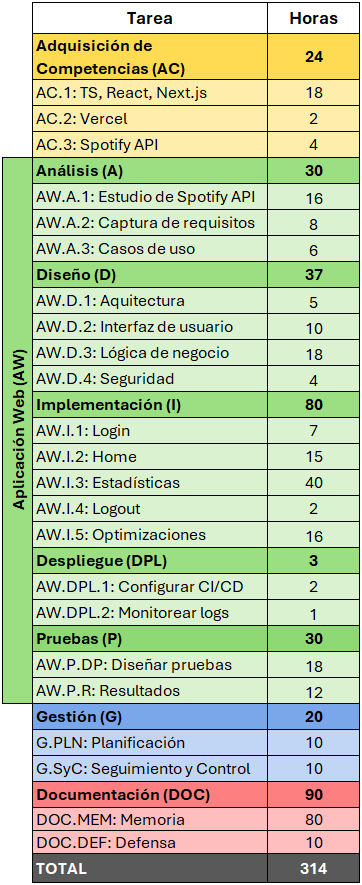
\includegraphics[width=0.55\textwidth]{figures/estimaciones_tareas.png}
    \caption{Tabla con las estimaciones de tiempo por paquete de trabajo y tarea del proyecto.}
    \label{tab:estimaciones_tareas}
\end{table}

\subsection{Dependencias entre Tareas}

En la figura \ref{fig:dependencias_tareas} se muestra un diagrama representando las dependencias que existen entre las diferentes tareas. De esta manera, se puede apreciar de forma visual las tareas que requieren la finalización de una o varias tareas para su comiezo.

\begin{figure}[H]
    \centering
    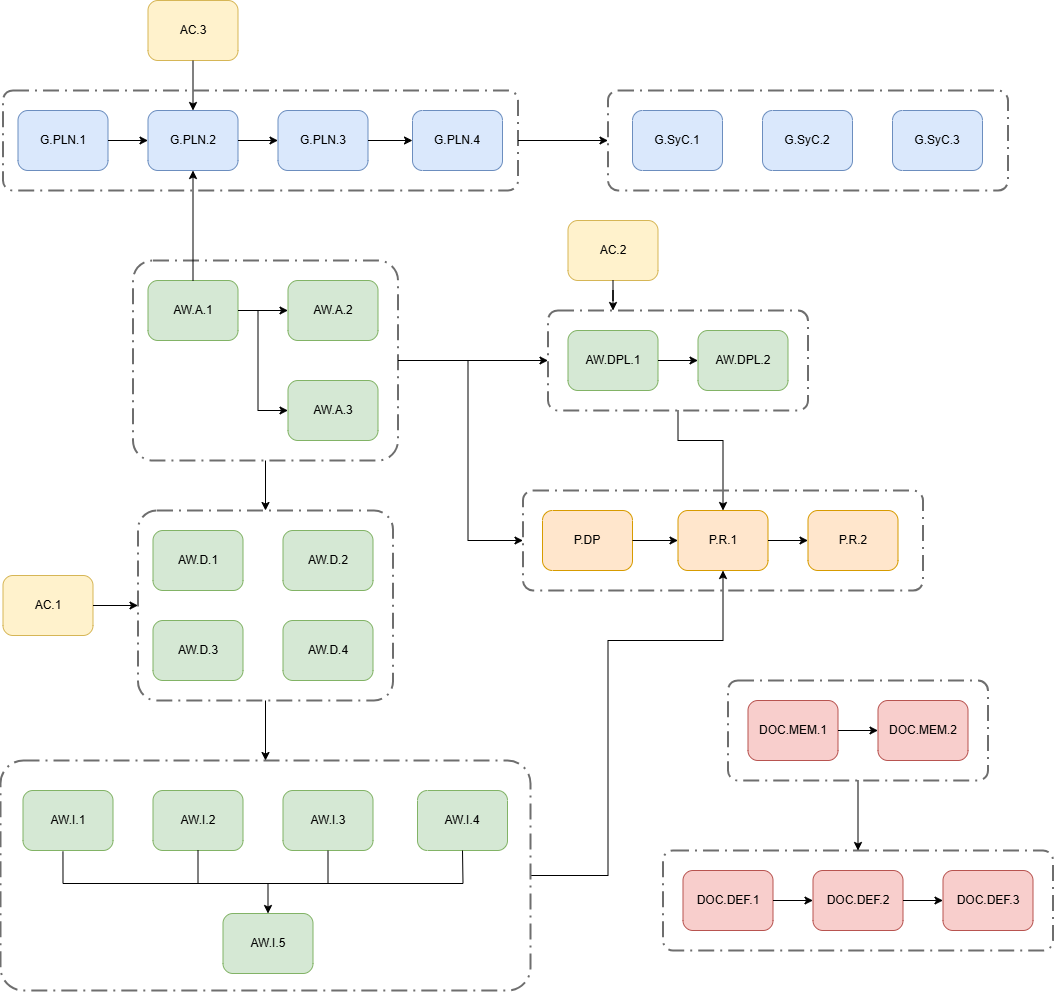
\includegraphics[width=\textwidth]{figures/dependencias_tareas.png}
    \caption{Diagrama de dependencias entre las tareas y paquetes de trabajo del proyecto.}
    \label{fig:dependencias_tareas}
\end{figure}

Como se puede apreciar, el proyecto debe iniciarse con las tareas de la planificación (paquete de trabajo \textbf{G.PLN}) y análisis (\textbf{AW.A}), al igual que el desarrollo de las tareas relacionadas con la memoria (\textbf{DOC.MEM}), que se realizan desde el inicio del proyecto hasta casi la finalización del TFG. Para ordenar temporalmente todas las tareas, en la siguiente sección se tratarán los periodos de desarrollo de cada una.

\subsection{Periodos de Desarrollo}


% * SEGUIR CON EL CRONOGRAMA O GANTT




\subsection{Hitos}






% TODO -> No está terminado, hay que revisar todos los riesgos y ponerlo bien
\section{Gestión de Riesgos}

% A continuación, se detallan los riesgos identificados que pueden afectar el desarrollo y el alcance del proyecto:

% \begin{itemize}
%     \item Dependencia de la API de \textit{Spotify}: La API de \textit{Spotify} podría cambiar, tener interrupciones o limitar el acceso a ciertos datos.

%     \item Limitaciones de la API de \textit{Spotify}: Restricciones en los tipos de datos accesibles, datos históricos limitados y permisos que los usuarios pueden no conceder.

%     \item Tasa de peticiones (\textit{rate limiting}) de la API de \textit{Spotify}: Exceder el número máximo de peticiones permitidas en un período de tiempo puede afectar la capacidad de actualización de datos en tiempo real.

%     \item Falta de almacenamiento persistente de datos del usuario: La imposibilidad de guardar datos entre sesiones limita ciertas funcionalidades como la personalización o el historial de preferencias del usuario.

%     \item Dependencia de servicios de terceros (\textit{Vercel}): Posibles interrupciones en los servicios de despliegue continuo o cambios en las políticas de \textit{Vercel}.

%     \item Tiempo limitado para el desarrollo: El tiempo y los recursos disponibles son finitos, lo que obliga a priorizar ciertas funcionalidades esenciales y descartar características adicionales.

%     \item Necesidad de conexión a Internet: La plataforma requiere una conexión a Internet activa para funcionar correctamente, lo que puede afectar a los usuarios en entornos con conectividad limitada.

%     \item Compatibilidad con navegadores y dispositivos antiguos: La plataforma puede no ser completamente funcional en navegadores o dispositivos más antiguos, lo que afecta a un porcentaje pequeño de usuarios.

%     \item Falta de experiencia con las tecnologías utilizadas: La curva de aprendizaje de tecnologías nuevas como \textit{Next.js} y \textit{TypeScript} podría ralentizar el desarrollo.

%     \item Rendimiento en dispositivos móviles o de gama baja: Las visualizaciones avanzadas pueden no funcionar de manera óptima en dispositivos con menor capacidad de procesamiento.

%     \item Seguridad y privacidad de los datos del usuario: El manejo incorrecto de los datos de los usuarios podría infringir las políticas de \textit{Spotify} o el RGPD, con consecuencias legales o de suspensión del servicio.

% \end{itemize}


% TODO -> Solo he pegado esto, pero hay que mirarlo todo
\section{Gestión de Calidad}

% El objetivo de la gestión de calidad es garantizar que el proyecto cumpla con los requisitos funcionales y no funcionales, asegurando un producto robusto, eficiente y alineado con las expectativas de los usuarios.

% \subsection{Línea Base}
% Los estándares mínimos establecidos para asegurar la calidad del proyecto son:
% \begin{itemize}
%     \item Buenas prácticas de desarrollo, aseguradas mediante revisiones de código.
%     \item Uso de metodologías ágiles para una planificación iterativa y control de calidad.
%     \item Diseño de interfaz de usuario intuitiva y conforme a los estándares de accesibilidad.
% \end{itemize}

% \subsection{Criterios de Éxito y Aceptación}
% Para asegurar que el producto cumple con las expectativas, los criterios de aceptación incluyen:
% \begin{itemize}
%     \item Cumplimiento de los requisitos funcionales y no funcionales.
%     \item Ausencia de errores críticos que afecten la experiencia de usuario.
%     \item Cumplimiento de los objetivos de rendimiento (tiempos de carga, capacidad de respuesta).
%     \item Feedback positivo en las pruebas de usabilidad realizadas con usuarios finales.
% \end{itemize}

% \subsection{Plan de Calidad}
% El plan de calidad incluye:
% \begin{itemize}
%     \item Pruebas automatizadas, incluyendo pruebas unitarias, de integración y de aceptación.
%     \item Revisión de código por pares para asegurar la consistencia y calidad del código.
%     \item Implementación de CI/CD usando Vercel para garantizar despliegues automáticos y controlados.
%     \item Pruebas de usabilidad con usuarios reales para validar la experiencia del usuario.
% \end{itemize}

% \subsection{Herramientas y Tecnologías}
% Para asegurar la calidad del proyecto, se utilizarán las siguientes herramientas:
% \begin{itemize}
%     \item \textbf{CI/CD}: Vercel y GitHub Actions para control de calidad durante el despliegue.
%     \item \textbf{Testing}: Jest para pruebas unitarias y Cypress para pruebas de integración.
%     \item \textbf{Control de calidad del código}: ESLint y Prettier para mantener estándares de código.
%     \item \textbf{Monitoreo del rendimiento}: Lighthouse para verificar tiempos de carga y rendimiento.
% \end{itemize}

% \subsection{Indicadores de Calidad}
% Los KPIs definidos para evaluar la calidad del proyecto son:
% \begin{itemize}
%     \item Número de bugs críticos detectados.
%     \item Tiempos de carga y respuesta del sistema.
%     \item Porcentaje de cobertura de pruebas.
%     \item Satisfacción del usuario en pruebas de usabilidad.
% \end{itemize}


% \section{Tecnologías y Herramientas Utilizadas}
